%-------------------------------------------------------------------------------
%                                PREAMBLE
%-------------------------------------------------------------------------------
\documentclass[usenames,dvipsnames,svgnames,10pt,aspectratio=169]{beamer}
%
\usefonttheme{professionalfonts}
% This theme uses TIKZ: compile twice with PDFLaTeX or LuaLaTeX.
%
%  Options:
%  - [clean]:    clean slides, i.e. logos and footbar are removed
%  - [kth]:      footbar style inspierd to the official KTH template
%  - [nicewave]: a different style of wave is used (not approved by FLOW)
%
\usetheme[clean]{flow}

\usepackage{tikz}
\usetikzlibrary{arrows}
\usetikzlibrary{shapes.geometric, math, positioning, calc, patterns, angles, quotes}
\usetikzlibrary{patterns.meta,decorations.pathmorphing}

\newcommand{\semaphore}[3]{% #1: color of circle,
                           % #2: color of semicircle
                           % #3: angle of semicircle 
  \tikz[node distance=0mm,baseline]
       {
         \node (s1) [circle, fill=#1, minimum size=6mm] {};
         \node      [semicircle, fill=#2, 
           inner sep=0pt, outer sep=0pt, minimum size=3mm,
           anchor=south,
           at={(s1.center)}, rotate=#3] {};
       }
}

\usepackage[]{circuitikz}

\usepackage{pgfplots}
\usepgfplotslibrary{polar}

\usepackage{hyperref,graphicx,lmodern}
\usepackage[utf8]{inputenc}
\usepackage{media9}
\usepackage{xcolor}
\usepackage{stmaryrd}
\usepackage{nicefrac}
\usepackage{multimedia}
\usepackage{multicol}
\usepackage{upgreek}
\usepackage[]{bm}
\usepackage[]{url}
\usepackage[]{animate}
\usepackage{amsmath}

\graphicspath{{imgs/}}
\setbeamertemplate{blocks}[rounded][shadow=true]

\DeclareMathOperator*{\maximize}{maximize~}

%-------------------------------------------------------------------------------
%                                TITLE PAGE
%-------------------------------------------------------------------------------
\title[Nonlinear physics] % Short title used in footline
{
	Linear systems
}

\author[J.-Ch.~Loiseau] % Presenting author in short form used in footline
{
	\underline{Jean-Christophe Loiseau}
}
% - Give the names in the same order as the appear in the paper.
% - Underline the presenting author.

\institute[unused]
{
	\url{jean-christophe.loiseau@ensam.eu} \\
	Laboratoire DynFluid \\
	Arts et M\'etiers, France.
}
% Keep it simple, no one is interested in your street address.

% University logo(s)
\logot{\includegraphics[width=.128\paperwidth]{DynFluid_logo}}  % Top logo
\logob{\includegraphics[width=0.128\paperwidth]{ENSAM_logo}} % Bottom logo
% \logoc[{\includegraphics[width=.128\paperwidth]{limsi}}]{\includegraphics[width=.128\paperwidth]{limsi}} % Corner logo
%
% Cover image: \cvrimg{x position}{y position}{cover image}
\cvrimg{.77}{.8}{\includegraphics[width=.4\paperwidth]{cover.png}}

\date[unused]{Physique non-lin\'eaire -- 2019-2020}

\begin{document}

\titleframe	% Print the title as the first slide

%-------------------------------------------------------------------------------
%                           PRESENTATION SLIDES
%-------------------------------------------------------------------------------

\begin{frame}[t, c]{First-order systems}{Flow on the real number line}
  \begin{minipage}{.48\textwidth}
    \begin{block}{\centering \textbf{First-order systems}}

    \[ \dot{x} = f(x, \mu) \]
    \end{block}

    \medskip

    \begin{itemize}
    \item $x(t)$ a real-valued function of time $t$,

      \medskip

    \item $f(x, \mu) : \mathbb{R} \times \mathbb{R} \to \mathbb{R}$ a smooth real-valued function of $x$ and $\mu$ and does not explicitely depend on time $t$.
    \end{itemize}
  \end{minipage}%
  \hfill
  \begin{minipage}{.48\textwidth}
    \[
    \begin{aligned}
      \dot{x} & = \mu \pm x^2 \\
      \dot{x} & = \mu x \pm x^2 \\
      \dot{x} & = \mu x \pm x^3 \\
    \end{aligned}
    \]
  \end{minipage}

  \vspace{1cm}
\end{frame}

\begin{frame}[t, c]{Two-dimensional systems}{Flow on the plane}
  \begin{minipage}{.58\textwidth}
    \begin{block}{\centering \alert{\textbf{Two-dimensional systems}}}
      \centering
      \(
      \begin{aligned}
        \dot{\bm{x}} = \bm{f}(\bm{x})
      \end{aligned}
      \)
    \end{block}

    \bigskip

    \begin{itemize}
    \item $\bm{x}(t) \in \mathbb{R}^2$ is a vector-valued function of time $t$.

      \bigskip

    \item $\bm{f} : \mathbb{R}^2 \to \mathbb{R}^2$ is a smooth vector-valued function of $\bm{x}$.

      \bigskip

    \item Again, $\bm{f}$ is autonomous, i.e. it does not depend explicitely on time.
    \end{itemize}
  \end{minipage}%
  \hfill
  \begin{minipage}{.38\textwidth}
    \centering
    \[
    \ddot{\theta} = -\dot{\theta} - \sin(\theta)
    \]
    \[
    \left\{
    \begin{aligned}
      \dot{x} & = x - y - (x^2 + y^2)x \\
      \dot{y} & = x + y - (x^2 + y^2)y
    \end{aligned}
    \right.
    \]
  \end{minipage}

  \vspace{1cm}
\end{frame}

\begin{frame}[t, c]{Two-dimensional systems}{Linear systems}
  \begin{minipage}{.68\textwidth}
    \begin{itemize}
    \item For today, we'll restrict our attention to \textbf{linear time invariant systems} of the form
      %
      \[
      \dot{\bm{x}} = \bm{Ax}
      \]
      %
      where $\bm{x} \in \mathbb{R}^2$ and $\bm{A} \in \mathbb{R}^{2 \times 2}$.

      \bigskip

    \item These typically result from linearizing the nonlinear system in the vicinity of a fixed point.

      \bigskip

    \item Our goal for today is to \textbf{classify} the possible dynamics in such simple systems.
    \end{itemize}
  \end{minipage}%
  \hfill
  \begin{minipage}{.28\textwidth}
    \centering
    \textbf{Linear systems}

    \[
    \dfrac{d}{dt} \begin{bmatrix} x \\ y \end{bmatrix}
    =
    \begin{bmatrix}
      a_{11} & a_{12} \\
      a_{21} & a_{22}
    \end{bmatrix}
    \begin{bmatrix}
      x \\ y
    \end{bmatrix}
    \]
  \end{minipage}

  \vspace{1cm}
\end{frame}

\begin{frame}[t, c]{Linear systems}{Analytic solution}
  \begin{minipage}{.58\textwidth}
    \begin{itemize}
      \item Given the initial condition $\bm{x}(0) = \bm{x}_0$, the analytical solution is given by
        %
        \[
        \bm{x}(t) = e^{t \bm{A}} \bm{x}_0
        \]
        %
        where $e^{t \bm{A}}$ is the matrix exponential.

        \bigskip

      \item Once again, the existence of an analytical solution provides little insights into what the dynamics look like.
    \end{itemize}
  \end{minipage}%
  \hfill
  \begin{minipage}{.38\textwidth}
    \centering
    \( e^{at} = 1 + at + \dfrac{(at)^2}{2!} + \dfrac{(at)^3}{3!} + \cdots \)

    \bigskip

    \( e^{t\bm{A}} = \bm{I} + t \bm{A} + \dfrac{(t \bm{A})^2}{2!} + \dfrac{(t \bm{A})^3}{3!} + \cdots \)
  \end{minipage}

  \vspace{1cm}
\end{frame}

\begin{frame}[t, c]{Linear systems}{Eigenvalues and eigenvectors}
  \begin{minipage}{.68\textwidth}
    Eigenvalues and eigenvectors are solution to the following equation
    %
    \[
    \bm{Av} = \lambda \bm{v}
    \]
    %
    which can be rewritten as
    %
    \[
    \left( \lambda \bm{I} - \bm{A} \right) \bm{v} = \bm{0}.
    \]
    
    Geometrically speaking, eigenvectors are left unchanged when multiplied by $\bm{A}$ except for a scaling $\lambda$.
  \end{minipage}%
  \hfill
  \begin{minipage}{.28\textwidth}
    \centering
    \textbf{Example}

    \bigskip

    \(
    \begin{bmatrix}
      2 & 1 \\ 1 & 2
    \end{bmatrix}
    \begin{bmatrix}
      1 \\ 1
    \end{bmatrix}
    =
    \begin{bmatrix}
      3 \\ 3
    \end{bmatrix}
    \)
  \end{minipage}

  \vspace{1cm}
\end{frame}

\begin{frame}[t, c]{Linear systems}{Eigenvalues and eigenvectors}
  \begin{minipage}{.68\textwidth}
    The equation $\left( \lambda \bm{I} - \bm{A} \right) \bm{v} = \bm{0}$ has non-trivial solutions if
    %
    \[
    \det \left( \lambda \bm{I} - \bm{A} \right) = 0.
    \]

    For a $2 \times 2$ matrix, this polynomial equation reduces to
    %
    \[
    \lambda^2 - \text{tr}(\bm{A}) \lambda + \det(\bm{A}) = 0
    \]
    %
    where $\text{tr}(\bm{A}) = a_{11} + a_{22}$ is the \textbf{trace} of $\bm{A}$ and $\det(\bm{A}) = a_{11}a_{22} - a_{21}a_{12}$ its \textbf{determinant}.
  \end{minipage}%
  \hfill
  \begin{minipage}{.28\textwidth}
    \centering
    \[
    \lambda_1 + \lambda_2 = \text{tr}(\bm{A})
    \]

    \[
    \lambda_1 \lambda_2 = \det(\bm{A})
    \]
  \end{minipage}

  \vspace{1cm}
\end{frame}

\begin{frame}[t, c]{Linear systems}{Eigenvalues and eigenvectors : tips and tricks}
  \begin{minipage}{.68\textwidth}
    \begin{itemize}
    \item If $\bm{A}$ is symmetric (i.e.\ $\bm{A} = \bm{A}^T$), then all of its eigenvalues are real.

      \bigskip

    \item If $\bm{A}$ is skew-symmetric (i.e.\ $\bm{A} = -\bm{A}^T$), then all of its eigenvalues are imaginary numbers.

      \bigskip

    \item Given the eigenvalues and eigenvectors, the matrix exponential $e^{t \bm{A}}$ is given by
      %
      \[
      e^{t \bm{A}} = \bm{V} e^{t \boldsymbol{\Lambda}} \bm{V}^{-1}
      \]
      %
      where $\left( e^{t \boldsymbol{\Lambda}} \right)_{ii} = e^{t \lambda_i}$.
    \end{itemize}
  \end{minipage}%
  \hfill
  \begin{minipage}{.28\textwidth}
    \centering
    \includegraphics[width=\textwidth]{Gears}
  \end{minipage}

  \vspace{1cm}
\end{frame}

\begin{frame}[t, c]{Linear systems}{Asymptotic fate of $\bm{x}(t)$}
  \begin{minipage}{.58\textwidth}

    Starting from $e^{t \bm{A}} = \bm{V} e^{t \boldsymbol{\Lambda}} \bm{V}^{-1}$, one can provide lower and upper bounds for $\| \bm{x}(t) \|_2^2 = \| e^{t \bm{A}} \bm{x}_0 \|_2^2$.

    \begin{overprint}
      \onslide<1>

      \medskip

      \[
      \| e^{t \boldsymbol{\Lambda}} \|_2^2 \leq \| e^{t \bm{A}} \|_2^2 \leq \| \bm{V} \|_2^2 \| \bm{V}^{-1} \|_2^2 \| e^{t \boldsymbol{\Lambda}} \|_2^2
      \]

      \bigskip

      \onslide<2>

      \medskip

      \[
      e^{2 t \Re(\lambda_1)} \leq \| e^{t \bm{A}} \|_2^2 \leq \kappa(\bm{A}) e^{2 t \Re(\lambda_1)}
      \]

      \bigskip

      The fate of $\bm{x}(t)$ is thus dictated by the real part of the leading eigenvalue.

      \begin{itemize}
      \item If $\Re(\lambda_1) > 0$, then $\| \bm{x}(t) \|_2 \to \infty$ as $t \to \infty$.
      \item If $\Re(\lambda_1) < 0$, then $\| \bm{x}(t) \|_2 \to 0$ as $t \to \infty$.
      \end{itemize}
    \end{overprint}
  \end{minipage}%
  \hfill
  \begin{minipage}{.38\textwidth}
    \begin{overprint}
      \onslide<1>
      \begin{center}
        \textbf{Vector-induced matrix norm}
      \end{center}
      \[
      \begin{aligned}
        \| \bm{G} \|_2 & = \max_{\bm{x}} \dfrac{\| \bm{Gx} \|_2}{\| \bm{x} \|_2} \\
        & = \sigma_1(\bm{G})
      \end{aligned}
      \]
      
      where $\sigma_1(\bm{G})$ is the leading singular value of $\bm{G}$.

      \onslide<2>
      \begin{center}
        \textbf{Vector-induced matrix norm}
      \end{center}

      If $\bm{G}$ is diagonal, then its 2-norm is
      %
      \[
      \| \bm{G} \|_2 = \max_i (\vert G_{ii} \vert).
      \]
      %
      where $G_{ii}$ is the diagonal entries of $\bm{G}$.

\end{overprint}
  \end{minipage}
    
  \vspace{1cm}
\end{frame}

\begin{frame}[t, c]{Linear systems}{What if the eigenvalues are imaginary ?}
  \begin{minipage}{.48\textwidth}
    Consider the harmonic oscillator
    %
    \[
    \ddot{x} + x = 0.
    \]

    Introducing the change of variable $y = \dot{x}$, it can be recast in matrix form as
    %
    \[
    \dfrac{d}{dt} \begin{bmatrix} x \\ y \end{bmatrix}
    =
    \underbrace{
      \begin{bmatrix}
        0 & 1 \\
        -1 & 0
      \end{bmatrix}
    }_{\bm{A}}
    \begin{bmatrix} x \\ y \end{bmatrix}
    \]
    %
    where $\bm{A}$ is skew-symmetric.
  \end{minipage}%
  \hfill
  \begin{minipage}{.48\textwidth}
    \centering
    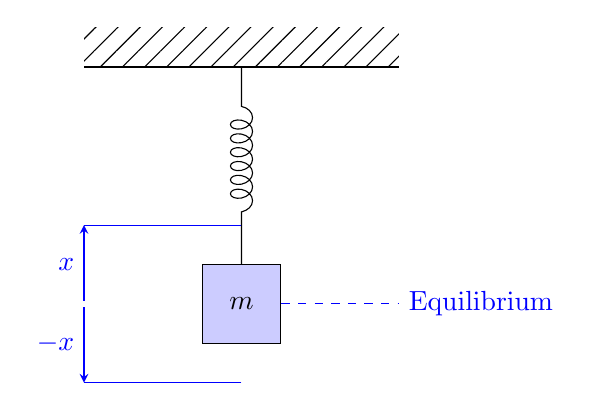
\begin{tikzpicture}[>=stealth]
      \path[pattern={Lines[angle=45,distance={8pt/sqrt(2)}]}] (-2, 5) edge ++(4,0) rectangle ++ (4, 0.5);

      \draw[decorate,decoration={coil, segment length=5pt, aspect=0.7, amplitude=4pt,
          pre=lineto, pre length=5mm, post=lineto, post length=5mm}] (0, 5) -- (0, 2.5)
      node[below, draw, minimum size=1cm, fill=blue!20] (m) {$m$};

      \draw[blue] (m.center-|0, 0) ++ (0, 1) -- ++ (-2, 0)
      edge[<-,edge label'=$x$,shorten >=1pt] (m.center-|-2, 0)
      (m.center-|0, 0) ++ (0, -1) -- ++ (-2, 0) 
      edge[<-,edge label=$-x$,shorten >=1pt] (m.center-|-2, 0)
      (m.east) edge[dashed] (m.east-|2, 0) 
      (m.east-|2, 0) node[right] {Equilibrium};
    \end{tikzpicture}
  \end{minipage}

  \vspace{1cm}
\end{frame}


\begin{frame}[t, c]{Linear systems}{What if the eigenvalues are imaginary ?}
  \begin{minipage}{.48\textwidth}
    Consider the harmonic oscillator
    %
    \[
    \ddot{x} + x = 0.
    \]

    Introducing the change of variable $y = \dot{x}$, it can be recast in matrix form as
    %
    \[
    \dfrac{d}{dt} \begin{bmatrix} x \\ y \end{bmatrix}
    =
    \underbrace{
      \begin{bmatrix}
        0 & 1 \\
        -1 & 0
      \end{bmatrix}
    }_{\bm{A}}
    \begin{bmatrix} x \\ y \end{bmatrix}
    \]
    %
    where $\bm{A}$ is skew-symmetric.
  \end{minipage}%
  \hfill
  \begin{minipage}{.48\textwidth}
    \centering
    \textbf{Solution}
    
    \medskip
    
    \( \det(\lambda \bm{I} - \bm{A}) = 0 \quad \Leftrightarrow \quad \lambda = \pm i \)
    
    \bigskip
    
    \[
    \begin{aligned}
      x(t) & = A \cos t + B \sin t \\
      & = A \cos(t + \phi)
    \end{aligned}
    \]
    
    \bigskip
    
    \begin{block}{}
      \centering
      \textbf{Oscillatory dynamics !}
    \end{block}
  \end{minipage}

  \vspace{1cm}
\end{frame}

\begin{frame}[t, c]{Linear systems}{What is the eigenvalues are complex ?}
  \begin{minipage}{.48\textwidth}
    Consider the harmonic oscillator with a small damping (i.e. $k < 1$)
    %
    \[
    \ddot{x} + 2k\dot{x} + x = 0.
    \]

    Introducing the change of variable $y = \dot{x}$, it can be recast in matrix form as
    %
    \[
    \dfrac{d}{dt} \begin{bmatrix} x \\ y \end{bmatrix}
    =
    \underbrace{
      \begin{bmatrix}
        0 & 1 \\
        -1 & -2k
      \end{bmatrix}
    }_{\bm{A}}
    \begin{bmatrix} x \\ y \end{bmatrix}
    \]
    %
    where $\bm{A}$ is no longer skew-symmetric.

  \end{minipage}%
  \hfill
  \begin{minipage}{.48\textwidth}
    \centering
    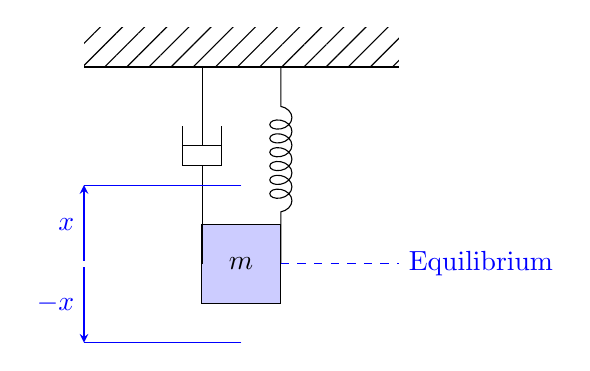
\begin{tikzpicture}[>=stealth]

      \path[pattern={Lines[angle=45,distance={8pt/sqrt(2)}]}] (-2, 5) edge ++(4,0) rectangle ++ (4, 0.5);

      \draw[decorate,decoration={coil, segment length=5pt, aspect=0.7, amplitude=4pt,
          pre=lineto, pre length=5mm, post=lineto, post length=5mm}] (0.5, 5) -- (0.5, 2.5)
      node[left, draw, minimum size=1cm, fill=blue!20] (m) {$m$};

      \draw[] (-0.5, 5) -- (-0.5, 4) {};
      \draw[] (-0.25, 4) -- (-0.75, 4) {};

      \draw[] (-0.5, 3.75) -- (-0.5, 2.5) {};
      \draw[] (-0.25, 3.75) -- (-0.75, 3.75) {};

      \draw[] (-0.25, 3.75) -- (-0.25, 4.25) {};
      \draw[] (-0.75, 3.75) -- (-0.75, 4.25) {};

      \draw[blue] (m.center-|0, 0) ++ (0, 1) -- ++ (-2, 0)
      edge[<-,edge label'=$x$,shorten >=1pt] (m.center-|-2, 0)
      (m.center-|0, 0) ++ (0, -1) -- ++ (-2, 0) 
      edge[<-,edge label=$-x$,shorten >=1pt] (m.center-|-2, 0)
      (m.east) edge[dashed] (m.east-|2, 0) 
      (m.east-|2, 0) node[right] {Equilibrium};
    \end{tikzpicture}    
  \end{minipage}

  \vspace{1cm}
\end{frame}

\begin{frame}[t, c]{Linear systems}{What is the eigenvalues are complex ?}
  \begin{minipage}{.48\textwidth}
    Consider the harmonic oscillator with a small damping (i.e. $k < 1$)
    %
    \[
    \ddot{x} + 2k\dot{x} + x = 0.
    \]

    Introducing the change of variable $y = \dot{x}$, it can be recast in matrix form as
    %
    \[
    \dfrac{d}{dt} \begin{bmatrix} x \\ y \end{bmatrix}
    =
    \underbrace{
      \begin{bmatrix}
        0 & 1 \\
        -1 & -2k
      \end{bmatrix}
    }_{\bm{A}}
    \begin{bmatrix} x \\ y \end{bmatrix}
    \]
    %
    where $\bm{A}$ is no longer skew-symmetric.

  \end{minipage}%
  \hfill
  \begin{minipage}{.48\textwidth}
    \centering
    \textbf{Solution}
    
    \medskip
    
    \( \det(\lambda \bm{I} - \bm{A}) = 0 \quad \Leftrightarrow \quad \lambda = -k \pm i \sqrt{1 - k^2} \)
    
    \bigskip
    
    \[
    \begin{aligned}
      x(t) & = A \cos(\sqrt{1 - k^2} t + \phi) e^{-kt}
    \end{aligned}
    \]
    
    \bigskip
    
    \begin{block}{}
      \centering
      \textbf{Exponentially decaying oscillations !}
    \end{block}
    
  \end{minipage}

  \vspace{1cm}
\end{frame}



\begin{frame}[t, c]{Linear systems}{What about the eigenvectors ?}
  \begin{minipage}{.58\textwidth}
    Vectors are geometrical objects and so eigenvectors will help us understand the solutions from a geometric point of view.

    \bigskip

    Consider the system
    %
    \[
    \dfrac{d}{dt} \begin{bmatrix} x \\ y \end{bmatrix}
    =
    \begin{bmatrix}
      1 & 1 \\
      4 & -2
    \end{bmatrix}
    \begin{bmatrix} x \\ y \end{bmatrix}.
    \]

    Its eigenvalues and eigenvectors are given by
    %
    \[
    \begin{aligned}
      \lambda_1 = 2, \quad & \lambda_2 = -3 \\
      \bm{x}_1 = \begin{bmatrix} 1 \\ 1 \end{bmatrix}, \quad & \bm{x}_2 = \begin{bmatrix} 1 \\ -4 \end{bmatrix}
    \end{aligned}
    \]
    %
    so the solutions to the system are $\bm{x}(t) = \alpha \bm{x}_1 e^{2t} + \beta \bm{x}_2 e^{-3t}$.
  \end{minipage}%
  \hfill
  \begin{minipage}{.38\textwidth}
    \centering
    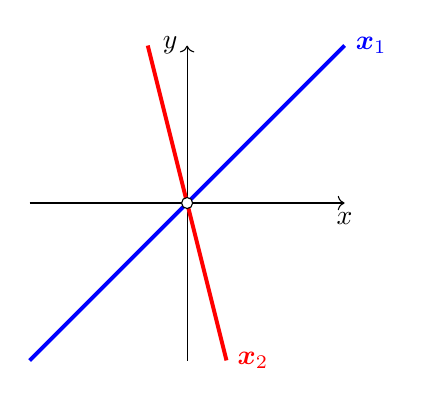
\begin{tikzpicture}

      \draw[->] (-2, 0) -- (2, 0) node[below] {$x$};
      \draw[->] (0, -2) -- (0, 2) node[left] {$y$};

      \draw[blue, line width=0.5mm, domain=-2:2] plot (\x, {\x}) node[right] {$\bm{x}_1$};
      \draw[red, line width=0.5mm, domain=-0.5:0.5] plot (\x, {-4*\x}) node[right] {$\bm{x}_2$};

      \node[circle, fill=white, draw=black, inner sep=0pt, minimum size=4pt] (a) at (0, 0) {};
    \end{tikzpicture}
  \end{minipage}

  \vspace{1cm}
\end{frame}

\begin{frame}[t, c]{Linear systems}{What about eigenvectors ?}
  \begin{minipage}{.58\textwidth}
    Let us explore the different kind of dynamics and phase portraits possible.
    For that, consider the system
    %
    \[
    \dfrac{d}{dt} \begin{bmatrix} x \\ y \end{bmatrix}
    =
    \begin{bmatrix}
      \mu & 0 \\
      0 & - 1
    \end{bmatrix}
    \begin{bmatrix} x \\ y \end{bmatrix}
    \]
    %
    and vary the parameter $\mu$.

    \bigskip

    In all cases, the eigenpairs are given by
    %
    \[
    \begin{aligned}
      \lambda_1 = \mu, \quad \lambda_2 = -1 \\
      \bm{x}_1 = \begin{bmatrix} 1 \\ 0 \end{bmatrix}, \quad \bm{x}_2 = \begin{bmatrix} 0 \\ 1 \end{bmatrix}.
    \end{aligned}
    \]
  \end{minipage}%
  \hfill
  \begin{minipage}{.38\textwidth}
    \begin{overprint}
      \onslide<1>
      \centering
      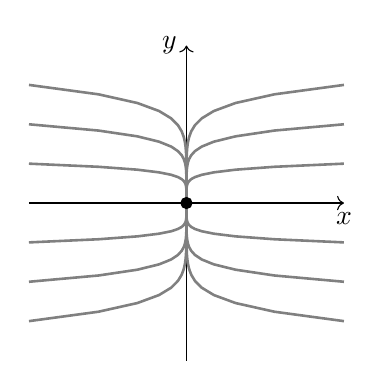
\begin{tikzpicture}
        \draw[->] (-2, 0) -- (2, 0) node[below] {$x$};
        \draw[->] (0, -2) -- (0, 2) node[left] {$y$}; 
       
        \draw[gray, line width=0.33mm, domain=0:2, variable=\t] plot ({2*exp(-7*\t)}, {1.5*exp(-\t)}) {};
        \draw[gray, line width=0.33mm, domain=0:2, variable=\t] plot ({2*exp(-7*\t)}, {exp(-\t)}) {};
        \draw[gray, line width=0.33mm, domain=0:2, variable=\t] plot ({2*exp(-7*\t)}, {0.5*exp(-\t)}) {};

        \draw[gray, line width=0.33mm, domain=0:2, variable=\t] plot ({2*exp(-7*\t)}, {-1.5*exp(-\t)}) {};
        \draw[gray, line width=0.33mm, domain=0:2, variable=\t] plot ({2*exp(-7*\t)}, {-exp(-\t)}) {};
        \draw[gray, line width=0.33mm, domain=0:2, variable=\t] plot ({2*exp(-7*\t)}, {-0.5*exp(-\t)}) {};

        \draw[gray, line width=0.33mm, domain=0:2, variable=\t] plot ({-2*exp(-7*\t)}, {1.5*exp(-\t)}) {};
        \draw[gray, line width=0.33mm, domain=0:2, variable=\t] plot ({-2*exp(-7*\t)}, {exp(-\t)}) {};
        \draw[gray, line width=0.33mm, domain=0:2, variable=\t] plot ({-2*exp(-7*\t)}, {0.5*exp(-\t)}) {};

        \draw[gray, line width=0.33mm, domain=0:2, variable=\t] plot ({-2*exp(-7*\t)}, {-1.5*exp(-\t)}) {};
        \draw[gray, line width=0.33mm, domain=0:2, variable=\t] plot ({-2*exp(-7*\t)}, {-exp(-\t)}) {};
        \draw[gray, line width=0.33mm, domain=0:2, variable=\t] plot ({-2*exp(-7*\t)}, {-0.5*exp(-\t)}) {};

        \node[circle, fill=black, draw=black, inner sep=0pt, minimum size=4pt] (a) at (0, 0) {};

      \end{tikzpicture}

      $$\vert \mu \vert \gg 1$$

      \onslide<2>
      \centering
      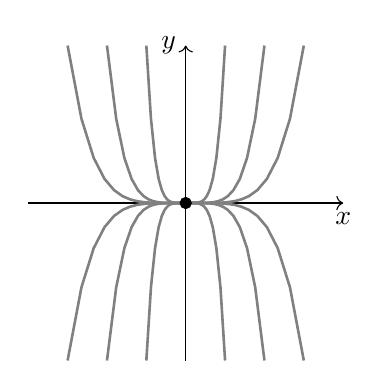
\begin{tikzpicture}
        \draw[->] (-2, 0) -- (2, 0) node[below] {$x$};
        \draw[->] (0, -2) -- (0, 2) node[left] {$y$}; 

        \draw[gray, line width=0.33mm, domain=0:15, variable=\t] plot ({1.5*exp(-0.2*\t)}, {2*exp(-\t)}) {};
        \draw[gray, line width=0.33mm, domain=0:15, variable=\t] plot ({exp(-0.2*\t)}, {2*exp(-\t)}) {};
        \draw[gray, line width=0.33mm, domain=0:15, variable=\t] plot ({0.5*exp(-0.2*\t)}, {2*exp(-\t)}) {};

        \draw[gray, line width=0.33mm, domain=0:15, variable=\t] plot ({1.5*exp(-0.2*\t)}, {-2*exp(-\t)}) {};
        \draw[gray, line width=0.33mm, domain=0:15, variable=\t] plot ({exp(-0.2*\t)}, {-2*exp(-\t)}) {};
        \draw[gray, line width=0.33mm, domain=0:15, variable=\t] plot ({0.5*exp(-0.2*\t)}, {-2*exp(-\t)}) {};

        \draw[gray, line width=0.33mm, domain=0:15, variable=\t] plot ({-1.5*exp(-0.2*\t)}, {2*exp(-\t)}) {};
        \draw[gray, line width=0.33mm, domain=0:15, variable=\t] plot ({-exp(-0.2*\t)}, {2*exp(-\t)}) {};
        \draw[gray, line width=0.33mm, domain=0:15, variable=\t] plot ({-0.5*exp(-0.2*\t)}, {2*exp(-\t)}) {};

        \draw[gray, line width=0.33mm, domain=0:15, variable=\t] plot ({-1.5*exp(-0.2*\t)}, {-2*exp(-\t)}) {};
        \draw[gray, line width=0.33mm, domain=0:15, variable=\t] plot ({-exp(-0.2*\t)}, {-2*exp(-\t)}) {};
        \draw[gray, line width=0.33mm, domain=0:15, variable=\t] plot ({-0.5*exp(-0.2*\t)}, {-2*exp(-\t)}) {};
       
        \node[circle, fill=black, draw=black, inner sep=0pt, minimum size=4pt] (a) at (0, 0) {};

      \end{tikzpicture}

      $$\vert \mu \vert \ll 1$$


      \onslide<3>
      \centering
      \begin{tikzpicture}
        \draw[->] (-2, 0) -- (2, 0) node[below] {$x$};
        \draw[->] (0, -2) -- (0, 2) node[left] {$y$}; 
       
        \node[circle, fill=black, draw=black, inner sep=0pt, minimum size=4pt] (a) at (0, 0) {};

      \end{tikzpicture}

      $$\vert \mu \vert \simeq 1$$

    \end{overprint}
  \end{minipage}
    
  \vspace{1cm}
\end{frame}

\begin{frame}[t, c]{Linear systems}{Classifying the fixed points}
  \begin{minipage}{.28\textwidth}
    Given the matrix $\bm{A}$, compute
    %
    \[
    \begin{aligned}
      \text{tr}(\bm{A}) & = a_{11} + a_{22} \\
      \det(\bm{A}) & = a_{11}a_{22} - a_{21}a_{12} \\
      \Delta & = \text{tr}^2(\bm{A}) - 4 \det(\bm{A})
    \end{aligned}
    \]
    %
    and classify the dynamics.
  \end{minipage}%
  \hfill
  \begin{minipage}{.68\textwidth}
    \centering
    \includegraphics[height=0.8\textheight]{fixed_points_classification}
  \end{minipage}
\end{frame}

\end{document}
